\section{Roles} The BI-DBS portal receives information about an authorized user from the study information system(KOS) based on the course information. The course information contains the identifier of the semester and the type of study program. Generally, there are eight user roles that are defined by the KOS for subjects and courses.\\

\noindent \textbf{KOS roles for subjects and their general description:}

\begin{itemize}
    \item \emph{Guarantor.} Guarantor is a course administrator. Thus a person with this role typically has all permissions across all course management.
    \item \emph{Examiner.} Examiners are responsible for managing and estimating students' exams. Therefore, this role would usually provide an access to exam materials and students' grades view and management.
    \item \emph{Editor.} Editor is a person who can edit the information about the subject. This role would provide an access to subject information management.
    \item \emph{Lecturer.} Lecturer role indicates that an individual with this role would need to be provided with access to manage course content including lectures, assignments and other study materials.
    \item \emph{Instructor.} Instructor is the role for teachers of exercises parallels. This role implies that a user needs permission to manage exercise materials and also estimate students' tests, semester works and other assignments.
    \item \emph{Laboratory instructor.} Laboratory instructor is an instructor who does teaching in the laboratories, which means that they may need to be provided with additional access to hardware and software management of the laboratory.
    \item \emph{Teacher.} The teacher is a general role for a person, who does teaching in the course. 
    \item \emph{Student.} It is a base role for students, that usually grants basic permissions to a user like access to their personal information, study program information and its resources, and also allows managing their projects and submitting assignments.
\end{itemize}

% % https://kosapi.fit.cvut.cz/projects/kosapi/wiki/Course


\noindent Two of those roles are not used for the BI-DBS portal. The first of them is the laboratory instructor, as the BI-DBS subject study program does not include laboratory exercises. The second one is the editor, the BI-DBS portal does not provide functionalities for changing the information about the subject. Therefore, we have a total of six roles used for permissions control in the current application.\\  
From these six roles in fact. Based on the feedback from the teachers and developers of the current BI-DBS portal and also my own research, we came to the conclusion that the access management system can be simplified by grouping the roles into three hierarchical layers.\\

\noindent \textbf{Reasons for simplifying the access management:}

\begin{enumerate}
    \item Based on the permissions research of the current project, I can report that most of the roles for teachers have the same or almost the same permissions. And the differences are insignificant.
    \item All the analyses and requirements of the BI-DBS portal designed by students including the theses are made for only three roles.
    \item Due to a lack of information about the roles developers often do not have a good understanding of all roles meaning and thus they tend to forget to permit success for some roles or confuse them with others.
\end{enumerate}

\noindent I am offering the simplification, which is based on grouping teaching roles that do not have significant permissions differences such as lecturer, examiner, instructor and teacher into one role. As I have already mentioned above, all the analyses are usually built on three roles where these 4 roles are taken as one role - teacher role, then there is a student and guarantor roles left which makes it a total of three.\\
After researching the functionalities and permissions structure of the current project and discussing the possible change with developers and managers, I came to the conclusion that it is absolutely safe to generalize the permissions for those four teacher roles. As the result, I got a new clear roles hierarchy, which is visualized in Figure 3.1.


\begin{figure}[h]
\centering
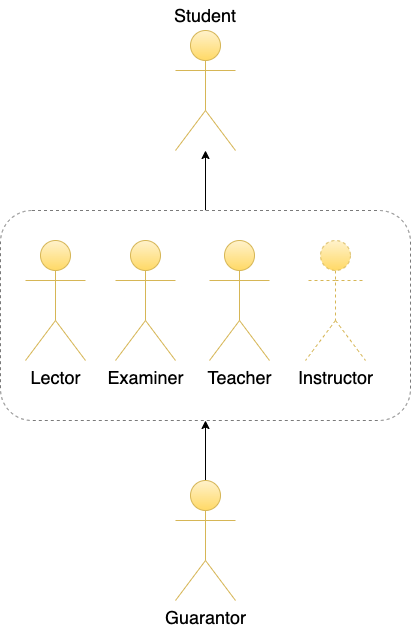
\includegraphics[scale=0.57]{../png/role.png}
\caption{Roles hierarchy}\label{picture:roles}
\end{figure}


\noindent Explaining the reason why the roles system must be hierarchical, I would start with 

% Beginning with a student role, which is the lowest layer I would like to explain why the roles must be hierarchical must be  All instructors, lectors, examiners, and also guarantors need to have an overview of how the whole application works including the students' side to be able to explain how to work with the portal, as well as they can use it for teaching. Therefore all the roles should have permission to access students .
